\section{Aufbau und Durchführung}
\label{sec:Durchführung}

\begin{figure}
    \centering
    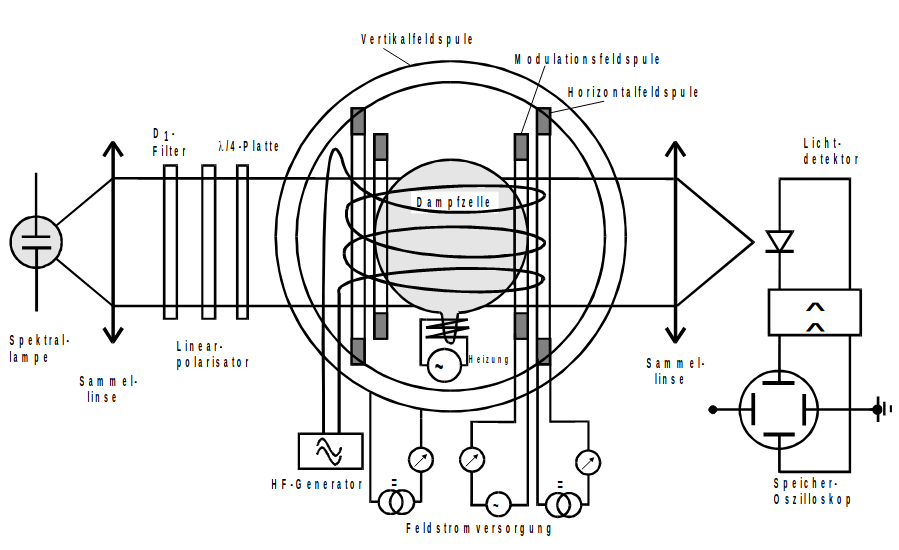
\includegraphics[width=\textwidth]{Fotos/aufbau.png}
    \caption{Der schematische Aufbau der genutzen Messapparatur \cite{V21}.}
    \label{fig:aufbau}
\end{figure}

Aus einer Rubidium-Licht-Quelle wird Licht 
mit der Wellenlänge $\lambda = \SI{794.8}{\nano \meter}$ erzeugt 
und mit einer Linse gebündelt.
Anschließend wird es mit einem Polarisationsfilter 
und einer $\lambda / 4$ - Platte zirkular polariert
und auf die Dampfzelle, die mit einem Offen geheitzt wird, gerichtet.
Hinter der Dampfzelle wird das Licht mit einer weiteren Linse gebündelt 
und über einen Lichtdetektor die Intensiät auf dem Oszilloskop dargestellt.
Um die Dampfzelle herum steht ein Helmholzspulenpaar ($R=\SI{15.79}{\cm}$, $N=154$), 
dass ein horizontales B-Feld erzeugt. 
Über den Helmholzspulen ist eine weitere Sweepspule gewickelt ($R=\SI{16.39}{\cm}$, $N=11$), 
die zum horizontalen Feld beisträgt.
Zudem verfügt der Aufbau über eine vertikale Spule zum Ausgleich des Erdmagnetfeldes ($R=\SI{11.735}{\cm}$, $N=20$).
\newline \newline
\noindent Zuerst wird die Apparatur justiert, um das Erdmagnetfeld auszugleichen. 
Hierzu wird der Ausgang der Sweepspule und die gemessene Intensiät der Diode 
auf dem Oszilloskop im XY-Modus angezeigt.
Es ist ein Peak zu sehen.
Die Ausrichtung der Apperatur und das vertikale B-Feld wird so lange variiert 
bis der Peak so schmal wie möglich ist.
\newline
\noindent Danach wird die RF-Frequenz von 100kHz bis 1 MHz in 100kHz-Schritten 
variiert und die Stärke des horizontalen B-Feldes bei den Resonatorfrequenzen gemessen.
Von einem dieser Messungen wird ein Foto gemacht, um daraus das Isotropenverhältnis zu bestimmen.
\newline
\noindent Als Letztes wird das RF-Feld an- and ausgeschaltet. 
Auf dem Oszilloskop wird im YT-Modus die Intensiät des Lichtes angezeigt.
Die Amplitude des RF-Feldes wird von 1V bis 10V in 1V-Schritten variiert 
und die Periodendauer der zusehenden Schwingung gemessen.

%Was wurde gemessen bzw. welche Größen wurden variiert?